\section{THEORY}

The necessary theory for understanding the numerical procedures and results are briefly explicated.

\subsection{Arrival Time}

In a Bohmian Mechanical formalism, the wave function and Schrödinger equation are foundational, just like in canonical formalisms, yet particles are dot-like entities which are \textbf{guided} by a pilot wave, making particles have a definite velocity and \textbf{trajectory}. Have a general wave function be written as
\begin{align}
    \Psi = \sqrt{\rho(\vec{r},t)} \cdot \text{exp}\left( i \frac{S(\vec{r},t)}{\hbar} \right),
\end{align}
where $\rho(\vec{r},t) = \Psi^*\Psi$ is the probability density of the wave function, and $S(\vec{r},t)$ its phase. One may now write the Bohmian velocity in the following form:
\begin{align}
\label{eq:velocityfield}
\vec{v} = \frac{\vec{j}(\vec{r}, t)}{\rho(\vec{r}, t)} = \frac{1}{m} \nabla S(\vec{r},t),
\end{align}
where $\vec{j}$ represents the probability current or \textbf{probability flux} of the wave function. The spatial variation of the wave function characterizes the probability flux of the wave function, and thus also its velocity. The arrival time of a particle in Bohmian Mechanics can be determined by following the motion of a particle's Bohmian trajectory, then registering the time at which the trajectory arrives at the detector:
\begin{align}
\frac{d}{dt} \vec{r}(t) = \vec{v} (\vec{r}(t), t) = \frac{|j(\vec{r}(t), t)|}{|\Psi(\vec{r}(t), t)|^2} \\
\Rightarrow \vec{r} = \vec{r}_0 + \int_0^t \vec{v} dt
\end{align}
Using the concept of Bohmian trajectories, the arrival time is the average traversal time across all these trajectories, having the trajectories start at $|\psi_0|^2$, and arrive or \textit{cross} a detector at an arbitrary path, plane or volume in the studied system (in this study, the detector). For this to hold, special requirements ought to be taken into consideration: the probability current needs to be strictly positive, and hence \textbf{backflow} of the trajectories needs to be eliminated (more on this in appendix \ref{ap:arrivaltime}), or at least: only the first crossing of a trajectory needs to considered. This is done by truncating the Bohmian trajectories (like in \cite{DAS2025170054}), or by using complex absorption potentials (similar to  Tumulka's approach in \cite{paper:tumulka}) at the boundaries of the numerical simulation. Both approaches are employed in this text. In any case, Bohmian trajectories justify the notion of using probability currents to describe an arrival time distribution, since it concerns itself with the \textbf{realism} of quantum mechanical systems, as opposed to only the \textbf{outcomes} of measurements as in canonical formalisms. For this to work, the previously mentioned conditions need to be met, which are summarised in the following box:
\fbox{%
  \begin{minipage}{0.46\textwidth}
  The probability density of the arrival time $t$ at a detector $\vec{r}_{\text{detector}}$ is given by:
    \begin{align}
    \label{eq:continuitity_1}
    \Pi(t) = - j(\vec{r}_{\text{detector}}, t)
    \end{align}
    iff the bohmian trajectories are strictly positive to one direction across the detector.
  \end{minipage}%
}
Studies \cite{MUGA2000353} \cite{Vona_2013} have shown that no POVM nor PVM exists for which $\langle \psi_0 | \hat{O_t} | \psi_0 \rangle = j(x=0, t)$ holds generally, however, the conditions in the boxed results are met in the studied free-fall setup, making the numerical setup feasible and physically meaningful. For a deep dive into the reasoning and setup of the boxed equation, please see appendix \ref{ap:arrivaltime}. The appendix also contains results and comparison of analytical solutions to the studied setup for weak delta barriers.

\subsection{Tunnelling Time}

In the Bohmian Mechanical picture, tunnelling time through a barrier is adequately defined due to the nature of \textbf{Bohmian trajectories}, and follows the same argument as for the arrival time in the previous section. Consider the setup as seen in figure \ref{fig:bohmian-tunnelling}, where a normalized Gaussian wave packet $\psi_0$ approaches a potential $V_0$.
\begin{figure}
    \centering
    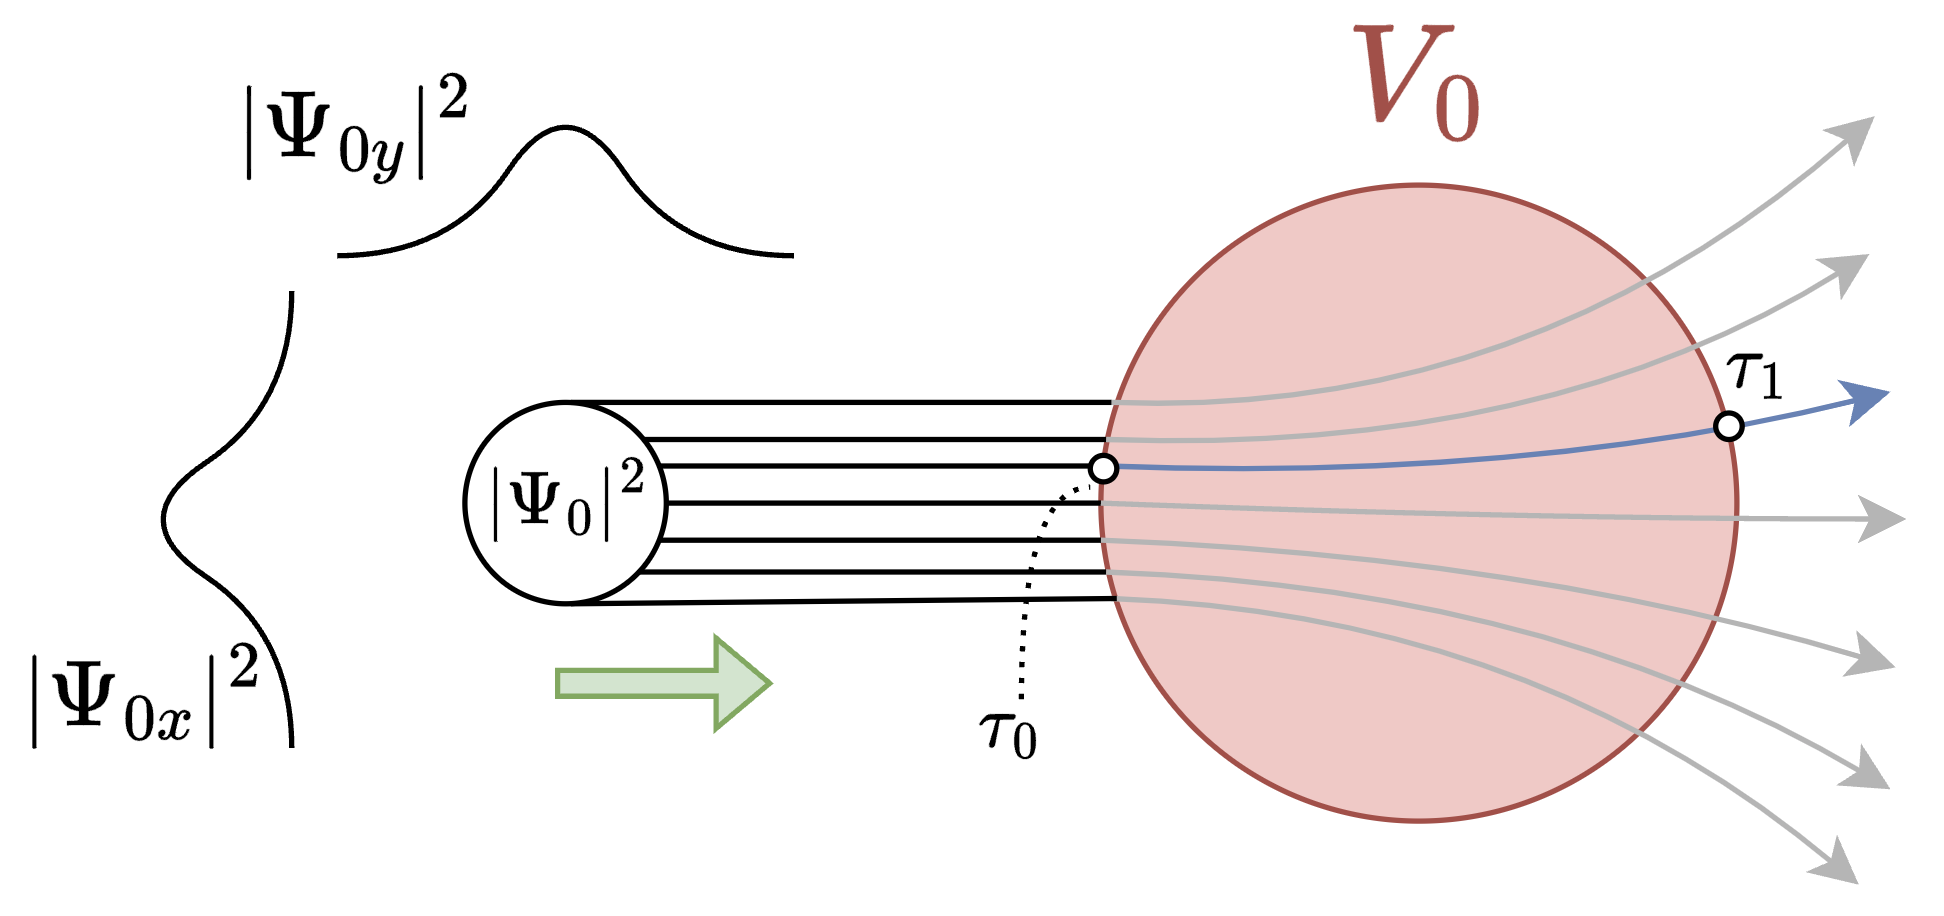
\includegraphics[width=1\linewidth]{Figures//tunneling_time_bohm.png}
    \caption{The tunnelling time on Bohmian trajectory is defined as $\tau_1 - \tau_0$, respectively the time of entering and exiting the barrier, in case the boundaries of the barrier are well-defined.}
    \label{fig:bohmian-tunnelling}
\end{figure}
Consider a Bohmian trajectory $\vec{Q}(t)$, which tunnels through the barrier of strength $V_0$. The tunnelling time of this trajectory equals to $\tau_{Q} = \tau_1 - \tau_0$, at least \textbf{if the boundary of the barrier is well-defined}. In the discussion section of this paper, it shall be discussed how Gaussian barriers have a not well-defined barrier, making the notion of tunnelling time inherently ambiguous in the Bohmian picture. In any case, the average tunnelling time of a quantum particle is the average tunnel time of N such Bohmian trajectories, which have been initialized in accordance to the wave function density distribution $|\psi_0|^2$:
\begin{align}
    \tau_t = \frac{1}{N} \sum_{i=0}^{N} \tau_{1}^{(i)} - \tau_{0}^{(i)}
\end{align}
Here too, backflow ought to be taken into consideration at the location of the idealised detector, and only the first crossing of the trajectory counts towards tunnelling time.
\subsection{Larmor Spin Precession And Larmor Clocks}
A classical electromagnetic result states that a dipole put in a uniform magnetic field $B_0$ will start precessing at the \textbf{Larmor frequency} due to the torque exerted on the dipole. This quantity is given by
\begin{align}
    \omega_L = \gamma B_0.
\end{align}
This classical result, applies to dipoles produced by quantum mechanical spin-$\frac{1}{2}$ particles. For electrons, $\gamma_e=-\frac{e}{2m_e}g_e$, with $g_e \approx2$, the electron g-factor, and $m_e$ the electron mass. For nuclei, $\gamma_n = \frac{e}{2 m_p}g$, with g the nuclear g-factor, and $m_p$ the proton mass. Bütticker argued in 1983 \cite{Buttiker1983LarmorClock} that spin-precession can be used to retrieve the \textit{dwell time} of a particle in a weak magnetic barrier, which is called the \textbf{Larmor Clock}. By shooting spin-$\frac{1}{2}$ particles through such magnetic fields, the expectation values of Pauli Spinors $\langle \sigma_x \rangle$ and $\langle \sigma_y \rangle$, in conjunction with the Larmor frequency, to retrieve an approximate \textbf{tunnelling time}. The main results are summarised in the box below:
\fbox{%
  \begin{minipage}{0.48\textwidth}
  \begin{align}
  \Theta(t) &\approx 
\tan^{-1}\!\Bigl(\,
\frac{\langle \sigma_y\rangle}{\langle \sigma_x\rangle}
\Bigr)\\
    \tau_{tunnelling} &= \frac{\Delta\Theta}{\gamma B_0} = \frac{\Delta\Theta}{\omega_L} \label{eq:tunnellingtimelarmoclcok}
\end{align}
  \end{minipage}%
}
Bütticker claimed that this result holds for any symmetric potentials of all kinds, in weak field regimes (including Gaussian ones) although the main derivation has been done using square potentials. The setup in this study assumes a uniform Gaussian magnetic field pointing in the positive z direction, which guarantees that the spin state remains in the xy-plane on the Bloch Sphere. \textbf{Larmor Clock} predictions are put against \textbf{Bohmian Tunnelling} predictions, and discussed. For a deeper treatment of the Larmor Clock, the reader is referred to appendix \ref{ap:larmorspinprecession}.